\chapter{Functional evaluation for vector / tensor data}
\label{chap:tensor-functional}

\begin{quote}
Spec dir:
\passthrough{\lstinline!specs/2026-05-05-phase-15-tensor-functional/!}.
Version: \passthrough{\lstinline!0.15.0!}.
\end{quote}

\subsection{What this gives you}\label{phase15-what}

Functional evaluation surface for \(\mathbf{u}\)-valued fields plus a
contraction expression-template (ET) layer that lets you assemble the
linear-elastic energy
\[
F[\mathbf u] \;=\; \int_\Omega \tfrac{1}{2}\,\boldsymbol{\sigma}:\boldsymbol{\varepsilon}\,dV,
\qquad
\boldsymbol{\varepsilon} = \tfrac12\!\big(\nabla\mathbf u + (\nabla\mathbf u)^\top\big),
\quad
\boldsymbol{\sigma} = \lambda\,\mathrm{tr}(\boldsymbol{\varepsilon})\,\mathbf{I}
                       + 2\mu\,\boldsymbol{\varepsilon},
\]
without ever materializing a \passthrough{\lstinline!Field<Mat3d>!}
intermediate for \(\boldsymbol{\sigma}\), \(\boldsymbol{\varepsilon}\),
or any linear combination thereof.

Three new public symbols (all under \passthrough{\lstinline!\\since 0.15.0!}):

\begin{itemize}
\tightlist
\item
  \passthrough{\lstinline!func::evaluate(Field<Vec3d>, callable)!} ---
  generalizes the Phase 4 / Phase 11 scalar surface to \(\mathbf
  u\)-valued inputs. Two SFINAE-detected callable arities:
  \passthrough{\lstinline!f(const Vec3d\& u)!} and
  \passthrough{\lstinline!f(const Vec3d\& u, const Mat3d\& grad\_u)!},
  with longest-arity-wins tie-break and the same
  \passthrough{\lstinline!Pairwise!}\,/\,\passthrough{\lstinline!Kahan!}
  reduction-tag dispatch as the scalar overloads. The rank-2 gradient
  follows the Phase 13 convention \(M(i, j) = \partial_j u_i\), so
  \(\mathrm{tr}(M) = \nabla\!\cdot\!\mathbf u\) by construction.
\item
  \passthrough{\lstinline!gridcalc::tensor::expr::*!} --- ten
  expression-template node types
  (\passthrough{\lstinline!Leaf!},
  \passthrough{\lstinline!IdentityField!},
  \passthrough{\lstinline!Scaled!},
  \passthrough{\lstinline!Plus!},
  \passthrough{\lstinline!Minus!},
  \passthrough{\lstinline!Mul!},
  \passthrough{\lstinline!Trace!},
  \passthrough{\lstinline!Sym!},
  \passthrough{\lstinline!SingleContract!},
  \passthrough{\lstinline!DoubleContract!}) plus operator overloads for
  \texttt{+}, \texttt{-}, unary \texttt{-}, scalar \texttt{*} / \texttt{/},
  and \texttt{*} between two scalar-valued expressions. The new header
  is \passthrough{\lstinline!include/gridcalc/tensor/Expressions.hpp!}.
\item
  \passthrough{\lstinline!func::integrate(expr, tag)!} --- new fused-loop
  overload accepting any contraction-ET node whose
  \passthrough{\lstinline!value\_type!} is \passthrough{\lstinline!double!}.
  Equivalent in numerical output to
  \passthrough{\lstinline!func::integrate(expr::materialize(expr), tag)!}
  but evaluates \passthrough{\lstinline!evalAt(i, j, k)!} cell-by-cell
  on the way to the reduction, so \passthrough{\lstinline!Mat3d!}
  intermediates never appear in memory.
\end{itemize}

Phase 13's eager
\passthrough{\lstinline!tensor::trace!}\,/\,\passthrough{\lstinline!tensor::singleContract!}\,/\,\passthrough{\lstinline!tensor::doubleContract!}
primitives are not modified --- the ET layer is a parallel surface, not
a replacement.

\subsection{Functional evaluation over \texorpdfstring{$\mathbf u$}{u}-valued fields}\label{phase15-evaluate}

The new overload mirrors the scalar one. Pass a
\passthrough{\lstinline!Field<Vec3d>!} and a callable; only the
gradient is materialized, and only when the 2-arg arity is selected:

\begin{verbatim}
#include <gridcalc/func/Functional.hpp>

const auto F = gridcalc::func::evaluate(u, [](const Vec3d& u_pt,
                                              const Mat3d& grad_u) {
    return u_pt.dot(u_pt) + grad_u.trace();
});
\end{verbatim}

The static-assert at the bottom of the dispatch ladder rejects callables
that cannot be invoked as \passthrough{\lstinline!f(Vec3d)!} or
\passthrough{\lstinline!f(Vec3d, Mat3d)!} with a return type
convertible to \passthrough{\lstinline!double!}. The
\passthrough{\lstinline!Order!} template parameter is intentionally
\emph{absent} on the new overload --- the scalar surface from
Phase 4 / Phase 11 also forwards to the default order-2 gradient, and
extending the new overload with a higher-order knob is one additive
overload to add later.

\subsection{The contraction expression-template layer}\label{phase15-et}

Phase 13 ships eager rank-2 contractions; each call allocates a fresh
\passthrough{\lstinline!Field<...>!}. The ET layer adds lazy nodes that
expose
\[
\texttt{evalAt(i, j, k)}\;=\;\text{the per-cell value the expression denotes,}
\]
plus a \passthrough{\lstinline!grid()!} accessor that returns the
shared underlying grid. Operators compose as you'd expect:

\begin{verbatim}
#include <gridcalc/tensor/Expressions.hpp>

namespace expr = gridcalc::tensor::expr;

Field<Mat3d> grad_u = gridcalc::diff::gradient(u);
auto eps          = expr::sym(expr::field(grad_u));
auto trace_eps    = expr::trace(eps);
auto integrand    = 0.5 * lambda * (trace_eps * trace_eps)
                  +       mu     * expr::doubleContract(eps, eps);
double F = gridcalc::func::integrate(integrand);
\end{verbatim}

No \passthrough{\lstinline!Field<Mat3d>!} is ever allocated for
\(\boldsymbol{\sigma}\) or \(\boldsymbol{\varepsilon}\); the only
heap allocation is the scalar integrand
\passthrough{\lstinline!Field<double>!} that
\passthrough{\lstinline!func::integrate!} reduces.

When you need the materialized field as input to a downstream operator,
\passthrough{\lstinline!expr::materialize(expr)!} is the explicit
escape hatch:

\begin{verbatim}
Field<Mat3d> eps_field = expr::materialize(expr::sym(expr::field(grad_u)));
\end{verbatim}

\subsubsection{Operator-overload coverage}

\begin{itemize}
\tightlist
\item
  \texttt{+}, \texttt{-} between two same-\passthrough{\lstinline!value\_type!}
  expressions.
\item
  Scalar \texttt{*} and \texttt{/} on either side of an expression.
\item
  Unary \texttt{-}.
\item
  \texttt{*} between two \passthrough{\lstinline!double!}-valued
  expressions (pointwise scalar multiply). Two
  \passthrough{\lstinline!Mat3d!}-valued expressions are intentionally
  not multiplied via \texttt{*}: the matrix product
  (\passthrough{\lstinline!singleContract!}) and the full contraction
  (\passthrough{\lstinline!doubleContract!}) need to be disambiguated
  at the call site.
\end{itemize}

\subsection{Worked example: linear elastic energy}\label{phase15-elastic-energy}

The roadmap acceptance bar is "elastic energy of a simple stretched
cubic block matches the analytical value." A literal rigid uniaxial
stretch \(u_x = \alpha\,x\) is \emph{not} periodic on
\([0, 2\pi]^3\) (it jumps from \(2\pi\alpha\) back to \(0\) across the
boundary), and Phase 1's only shipped boundary policy through
Phase 14 is \passthrough{\lstinline!IndexPolicy::Periodic!}. The
periodic substitute is the \emph{uniaxial dilation wave}
\[
\mathbf u(x, y, z) \;=\; \big(\alpha\sin(k_0 x),\,0,\,0\big),\qquad k_0 = 1
\]
on the standard \([0, 2\pi]^3\) box. The strain is diagonal,
\(\varepsilon_{xx}(x) = \alpha\cos(k_0 x)\) and zero elsewhere; the
elastic-energy density follows:
\[
\tfrac12\,\boldsymbol{\sigma}:\boldsymbol{\varepsilon}
\;=\;
\tfrac12\,(\lambda + 2\mu)\,\alpha^2\cos^2(k_0 x).
\]
Integrating over the box,
\[
F_{\mathrm{ref}}
\;=\;
\tfrac12\,(\lambda + 2\mu)\,\alpha^2
\,\bigl[\textstyle\int_0^{2\pi}\!\cos^2(k_0 x)\,dx\bigr]\,(2\pi)^2
\;=\;
2\pi^3\,(\lambda + 2\mu)\,\alpha^2.
\]
Phase 19 will unlock literal rigid-stretch geometries via the
\passthrough{\lstinline!Dirichlet!} / \passthrough{\lstinline!Neumann!}
boundary policies; until then this periodic wave is the right
substitute. The closed-form constant
\(2\pi^3(\lambda + 2\mu)\alpha^2\) is the reference the acceptance
test compares against.

\subsubsection{Helpers}

\passthrough{\lstinline!examples/common/elastic_energy.hpp!} exposes
four helpers (under
\passthrough{\lstinline!gridcalc::examples::elastic_energy!}):

\begin{itemize}
\tightlist
\item
  \passthrough{\lstinline!lameFromYoungPoisson(E, nu)!} ---
  \((\lambda, \mu)\) from engineering constants.
\item
  \passthrough{\lstinline!makeUniaxialPeriodicDisplacement(grid, alpha, axis)!}
  --- builds the \(\mathbf u\) field above for any of the three axes.
\item
  \passthrough{\lstinline!linearElasticEnergyDensity(lambda, mu, grad_u)!}
  --- returns the per-point Lamé closed form
  \(\tfrac12(\lambda\,\mathrm{tr}(\boldsymbol\varepsilon)^2
  + 2\mu\,\boldsymbol\varepsilon:\boldsymbol\varepsilon)\), matching
  the \passthrough{\lstinline!func::evaluate!} 2-arg signature.
\item
  \passthrough{\lstinline!analyticalLinearElasticEnergy(grid, alpha, lambda, mu, axis)!}
  --- the closed-form constant above. Throws if the grid isn't the
  standard \([0, 2\pi]^3\) box.
\end{itemize}

\subsubsection{Acceptance test}

\passthrough{\lstinline!test/elastic_energy_test.cpp!}
discharges the roadmap bar at \(N = 64\),
\(E = 1\),
\(\nu = 0.3\),
\(\alpha = 0.01\): relative error
\(|F_h - F_{\mathrm{ref}}| / |F_{\mathrm{ref}}| < 5\times 10^{-3}\)
(measured \(\approx 3.2\times 10^{-3}\) at this grid size, with the
order-2 leading constant of \(\sim 0.3\)). A separate
convergence sweep on \(N \in \{16, 32, 64\}\) verifies the rate sits
in the \([1.6, 2.4]\) band on \(\log\)-\(\log\) of error vs.\ \(h\).

\subsection{Demo binary: \texttt{examples/elastic\_energy.cpp}}\label{phase15-demo}

CLI options: \passthrough{\lstinline!--n-x!},
\passthrough{\lstinline!--young!}\,/\,\passthrough{\lstinline!--nu!}
(default \(E=1, \nu=0.3\)), or \passthrough{\lstinline!--lambda!} /
\passthrough{\lstinline!--mu!} to override the Lamé constants
directly, \passthrough{\lstinline!--alpha!} (default 0.01),
\passthrough{\lstinline!--axis x|y|z!}, and
\passthrough{\lstinline!--out-dir!}. Prints \(F_h\), \(F_{\mathrm{ref}}\),
the relative error, and the wall time, then writes a single VTK
snapshot of the axial-strain field
\(\varepsilon_{\text{axis,axis}}\) for inspection in ParaView / VisIt.

\begin{center}
  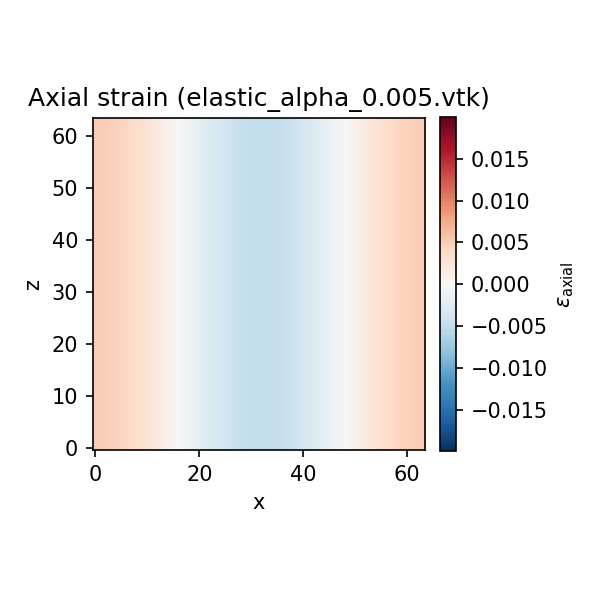
\includegraphics[width=0.32\linewidth]{figures/elastic-energy/small.png}\hfill
  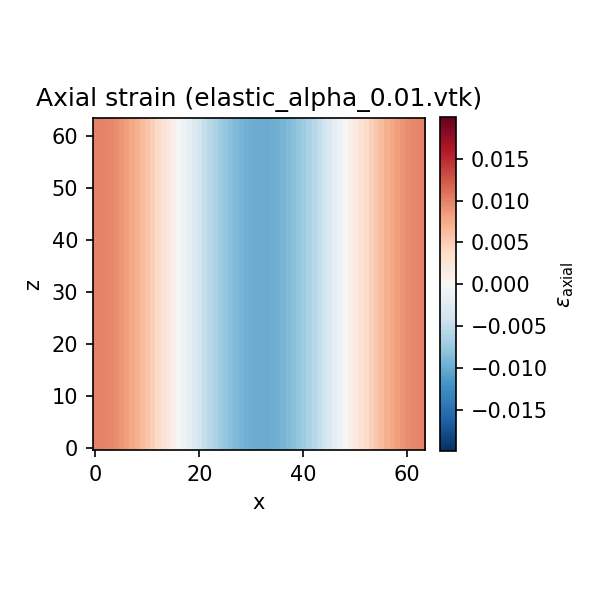
\includegraphics[width=0.32\linewidth]{figures/elastic-energy/medium.png}\hfill
  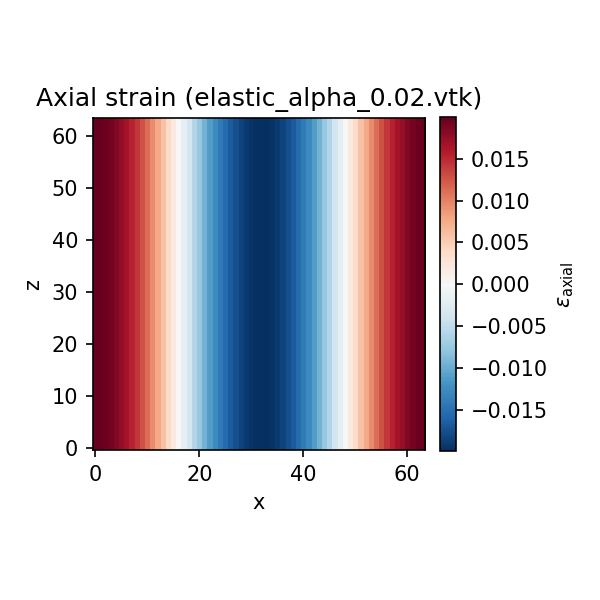
\includegraphics[width=0.32\linewidth]{figures/elastic-energy/large.png}
\end{center}
\noindent
\textit{Axial-strain \(\varepsilon_{xx}\) at \(N = 64\) for
\(\alpha \in \{0.005, 0.01, 0.02\}\) (left to right). Color limits are
shared across the three panels so the amplitude scaling is visible
directly.}

The demo binary lives behind
\passthrough{\lstinline!GRIDCALC_BUILD_EXAMPLES=ON!} (the default in
CI), mirroring the Phase 12 CH and Phase 14 heterogeneous-diffusion
patterns. CI does not run the binary; the
\passthrough{\lstinline!ElasticEnergyDemoTest!} static-cached gate in
\passthrough{\lstinline!test/elastic_energy_demo_test.cpp!} runs an
\(N=24\) version on every PR with a 5\,\% relative-error gate.

\subsection{What this does \emph{not} do}\label{phase15-not}

\begin{itemize}
\tightlist
\item
  No rank-3 / rank-4 tensor types. The
  \passthrough{\lstinline!Eigen::TensorFixedSize!} portability risk
  recorded under STATUS.md "Open / deferred items" stays deferred.
\item
  No \passthrough{\lstinline!gradient(Field<Mat3d>)!} or
  \passthrough{\lstinline!func::evaluate(Field<Mat3d>, ...)!}, since
  both consume rank-3 outputs.
\item
  No literal rigid-stretch demo on \([0, L]^3\). Periodicity-only.
  Phase 19 lifts this restriction.
\item
  No nonlinear / hyperelastic / anisotropic models, no 4th-order
  stiffness \(C_{ijkl}\), no plasticity, no fracture.
\item
  No SIMD / OpenMP / cache-blocking on the ET layer ---
  Phase 21's performance pass.
\end{itemize}
